\documentclass{article}
\usepackage{graphicx}
\usepackage{amsmath}

\begin{document}

\title{Graphics Pipeline}
\author{Justin Huffman, Eryn Kelsey-Adkins, Jesus Torres}

\maketitle

\begin{abstract}
The rendering pipeline is theseries of steps a graphics system needs to follow to render a 3D scene to a 2D screen. These steps start with the Application, then the Geometry, the Rasterization, and finally the Display. This presentation provides a brief overview of each of the steps and the matrices used to transform 3D objects into 2D displays.
\end{abstract}

\section{Introduction}
Here is the text of your introduction.

\section{Application: how 3D models are stored}
\subsection{Face-Vertex Mesh}
\subsubsection{Face List}
A list of faces (triangles), with each face being defined by the three vertices that make it up.

\subsubsection{Vertex List}
List of vertices (points in 3D space), with each vertex being defined by its x, y, and z coordinates, as well as a list of faces that it belongs to. This is redundant, but saves having to search the face list.

\subsection{Homogeneous Coordinates}
Imagine a 2D projector. The X and Y values are easy to see, but what happens to the image as you move the projector closer or further away from the screen? The image is scaled up or down. This is the W value in homogeneous coordinates.\footnote[1]{https://www.tomdalling.com/blog/modern-opengl/explaining-homogenous-coordinates-and-projective-geometry/} All vertices and vectors are in homogenous (x, y, z, w) form. At this time, W = 1 for vertices (points in space) and W = 0 for vectors (directions and facings). Other values of W are used in later steps for projection. The use of homogeneous vectors allows for standard 4x4 matrices to be used to transform both vertices and vectors.

\subsection{Model/World Transformation}
\subsubsection{World Coordinate System}
The world coordinates are the bedrock of the 3D model. This universal coordinate system is independent of the camera and objects or primatives, which each have their own coordinate system, are placed within the world coordinates. Every point is defined by three vertices $(x, y, z)$. The cartesian coordinates can be left- or right- handed, defined by whether the z vertex points into or out of the display./footnote[1]{cs.uic.edu} Depending on the coordinate system being used, the models may need to be inverted when loading for veiwing.

\begin{figure}
    \centering
    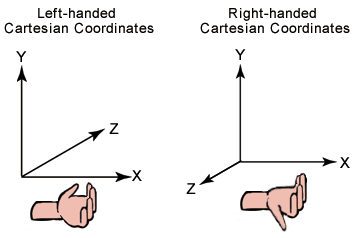
\includegraphics[width=3.0in]{leftrght.png}
    \caption{Left- and Right- Handed Cartesian Coordinates}
    \label{LeftRight}
\end{figure}

\subsubsection{Object Coordinate System}
As mentioned above, each object has its own set of coordinates. Objects are most often represented by polyhedren, further broken down into triangles. Each triangle is defined, counterintuitively, by 4 vertices: the 3 edges, and a fourth vertex defining the front of the primative. When objects are moved in relation to the world coordinates, the origin of the object (in the object's coordinate system) is moved, with all other points transformed and equal amount.

\paragraph
Objects can further have a hierarchal coordinate system. The University of Illinois uses the example of a hand being positioned relative to the arm, rather than to the world coordinate system. 

\subsection{Camera Transformation}
The camera transformation can be thought of as one more coordinate system: based upon the viewpoint of the observer, changing as the point of view changes. This coordinate system is defined  by:

\begin{itemize}
\item A scene of the world coordinates, including all primatives within those coordinates
\item The camera position - $C = (x_{c}, y_{c}, z_{c})$
\item The point of the camera's focus - $A = (x_{a}, y_{a}, z_{a})$
\item The field of view angle - $\alpha$
\item The definition of the near and far planes, perpindicular to A with a distance of n and f from the camera
\end{itemize}

A pyramid is formed with C, A, and $\alpha$ which is then truncated by n and f into a frustum.

The transformation of the truncated viewing volume is given by:

\[A_{\alpha, n, f} = 
\begin{pmatrix}
\cot \frac{\alpha}{2} & 0 & 0 & 0 \\
0 & \cot \frac{\alpha}{2} & 0 & 0 \\
0 & 0 & \frac{f+n}{f-n} & -1 \\
0 & 0 & \frac{2fn}{f-n} & 0
\end{pmatrix}\]

\footnote[1]{http://idav.ucdavis.edu/education/GraphicsNotes/Viewing-Transformation/Viewing-Transformation.html\#matrix}

\section{Geometry}

\subsection{Projection}
Projection transforms the view volume into a unit cube with extreme points at (1, 1, 1) and (-1, -1, -1). This step is called projection even though it is a volume to volume transformation because the z-coordinate is saved for the rasterization step.

\subsubsection{Types of Projection}

\begin{figure}
    \centering
    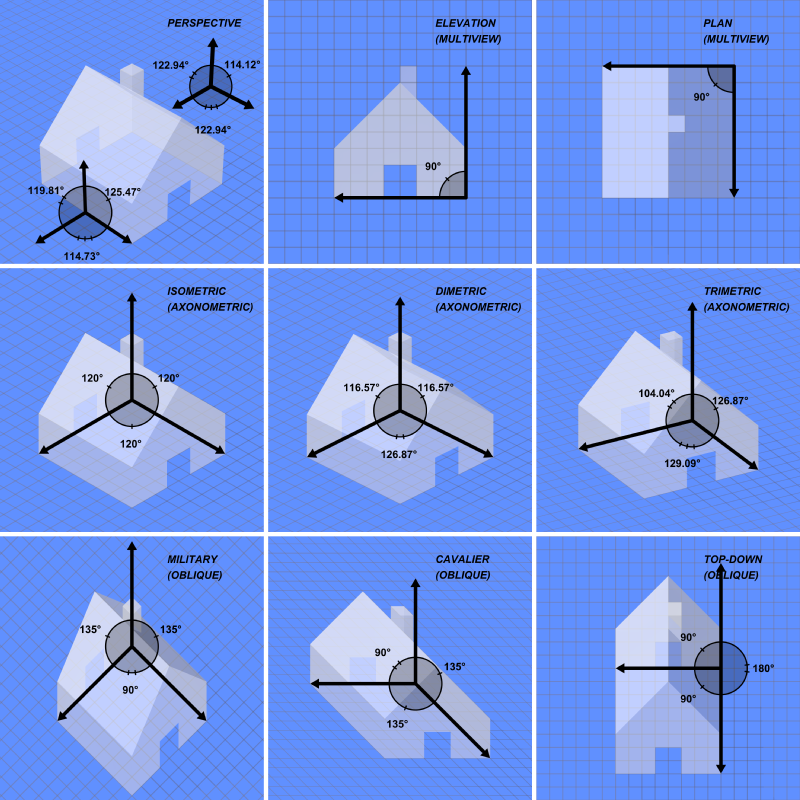
\includegraphics[width=3.0in]{Graphical_projection_comparison.png}
    \caption{A comparison of projection types}
    \label{projectiontypes}
\end{figure}

\subsubsection{Orthographic Projection}
Orthographic projection is mostly used in engineering for multi-view drawings. It is to scale, and all parallel line remain parallel with no forced perspective. An orthographic projection transformation can be represented as

\[ P = \begin{pmatrix}
  1 & 0 & 0 & 0 \\
  0 & 1 & 1 & 1 \\
  0 & 0 & 0 & 0 \\
  0 & 0 & 0 & 1 
 \end{pmatrix}\]	

Each homogeneous vector $v = (v_x, v_y, v_z, 1)$, the transformed vector would be

\[P_{v} = \begin{pmatrix}
  1 & 0 & 0 & 0 \\
  0 & 1 & 1 & 1 \\
  0 & 0 & 0 & 0 \\
  0 & 0 & 0 & 1 
 \end{pmatrix}	
*
\begin{pmatrix}
  v_{x} \\
  v_{y} \\
  v_{z} \\
  1
 \end{pmatrix}	
=
\begin{pmatrix}
  v_{x} \\
  v_{y} \\
  0 \\
  1
 \end{pmatrix}\]

\subsubsection{Weak Perspective Projection}
Weak perspective projection adds a scaling factor to orthographic projection. This scaling factor uses averages to apporximate perspective and is used with simple models and small fields of view.

  \[P_{x} =  \frac{X}{Z_{ave}}\]
  \[P_{y} =  \frac{Y}{Z_{ave}}\]

assuming focal length $f = 1$.

\subsubsection{Perspective Projection}
Perspective projection most closely replicates the human binocular vision where distant objects appear smaller. To describe the transformation, we must start with four variables:

\begin{itemize}
  \item $a_{x, y, z}$ - the 3D position of a point A that is to be projected
  \item $c_{x, y, z}$ - the 3D position of a point C representing the camera
  \item $\theta_{x, y, z}$ - the orientation of the camera
  \item $e_{x, y, z}$ - the display surface's positon relative to the camera pinhole. (Although negative z values are more correct, the create an inverted image both horizontally and vertically, so most conventions use positive values.
\end{itemize}

To compute the 2D projection ($b_{x, y}$) of the point A ($a_{x, y, z}$) that is to be projected, a vector $d_{x, y, z}$ is first defined as the position of point A with respect to the camera transformation, with origin in C and rotated by $\theta$:

\[\begin{pmatrix}
  d_{x} \\
  d_{y} \\
  d_{z} 
 \end{pmatrix}
=
\begin{pmatrix}
  1 & 0 & 0 \\
  0 & \cos(\theta_{x}) & \sin(\theta_{x}) \\
  0 &  -\sin(\theta_{x}) & \cos(\theta_{x}) 
 \end{pmatrix}
\begin{pmatrix}
  \cos(\theta_{y}) & 0 & -\sin(\theta_{y}) \\
  0 & 1 & 0 \\
  \sin(\theta_{y}) & 0  & \cos(\theta_{y}) 
 \end{pmatrix}\
\begin{pmatrix}
  \cos(\theta_{z}) & \sin(\theta_{z})  & 0  \\
  -\sin(\theta_{z}) & \cos(\theta_{z}) & 0 \\
  0 & 0  & 1 
 \end{pmatrix}\
\left(
\begin{bmatrix}
  a_{x} \\
  a_{y} \\
  a_{z} 
\end{bmatrix}\
-
\begin{bmatrix}
  c_{x} \\
  c_{y} \\
  c_{z} 
\end{bmatrix}\
\right)\]

\subsection{Clipping}
Clipping saves time and energy by specifying only those objects within the view volume for rendering. The vidual unit cube has been transformed into a truncated pyramid (frustrum) and objects outside of the frustrum are discarded by a method appropriately named frustrum culling. Objects that will be obscured by other primatives are also culled through backface culling. Objects inside the frustum are saved for rasterization.
\paragraph
Objects that intersect the edges of the frustrum must be clipped. Line clipping simply modifies the endpoints of lines to lie within the appropriate rectangle. Polygon clipping converts a polygon that intersects the frustum into one or more polygons the form the intersection of the original with the clip window. The Sutherland-Hodgman Polygon Clipping Algorithm is commonly used\footnote[2]{https://www.geeksforgeeks.org/polygon-clipping-sutherland-hodgman-algorithm-please-change-bmp-images-jpeg-png/}:

\begin{figure}
    \centering
    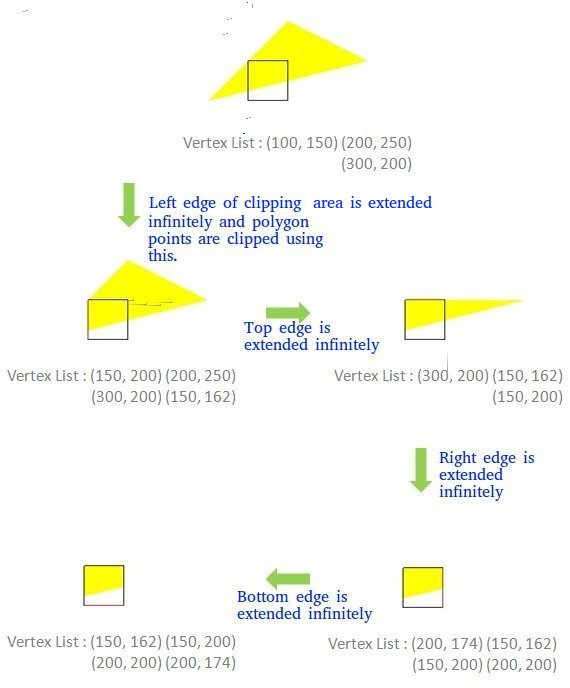
\includegraphics[width=3.0in]{Sutherland-Hodgman-Example.jpg}
    \caption{An example of the Sutherland-Hodgman Algorithm in use}
    \label{Sutherland-Hodgman}
\end{figure}

\subsection{Window-Viewport Transformation}
Translates camera coordinated into screen coordinated in order to match the size and location of the window

\subsection{Rasterization}
Converts primitives (shapes) to discrete coordinates (pixels)

\subsubsection{Bresenham's line algorithm}
Draws line between two points in pixels

\subsubsection{Z-buffering}
Solves visibility problem
\section{Conclusion}
Write your conclusion here.

\end{document}